\subsection{Experimental Setup}
\label{sec:setup}

\subsubsection{System used}

We conduct experiments on a system equipped with an AMD EPYC-7742 processor, with $64$ cores and operating at a frequency of $2.25$ GHz. Each core has a $4$ MB L1 cache, a $32$ MB L2 cache, and shares a $256$ MB L3 cache. The server is configured with $512$ GB of DDR4 system memory and operates on Ubuntu $20.04$.


\subsubsection{Configuration}

We employ 32-bit integers for vertex ids and 64-bit floating-point numbers for vertex rankings. To denote affected vertices, an 8-bit integer vector is utilized. The rank computation utilizes OpenMP's \textit{dynamic schedule} with a chunk size of $2048$, facilitating dynamic workload balancing among threads. We use a damping factor of $\alpha = 0.85$ \cite{rank-langville06}, an iteration tolerance of $\tau = 10^{-10}$ using the $L_\infty$-norm \cite{rank-dubey22, rank-plimpton11}, and limit the maximum number of iterations (\texttt{MAX\_ITERATIONS}) to $500$ \cite{nvgraph}. We run all experiments with $64$ threads to match the number of cores available on the system (unless specified otherwise). Compilation is performed using GCC $9.4$ and OpenMP $5.0$.


\subsubsection{Dataset}

We use four graph classes sourced from the \textit{SuiteSparse Matrix Collection} \cite{suite19}, as detailed in Table \ref{tab:dataset}. The number of vertices in these graphs range from $3.07$ million to $214$ million, with edge counts spanning from $37.4$ million to $1.98$ billion. To address the impact of dead ends (vertices lacking out-links), a global teleport rank contribution is computed in each iteration. We mitigate this overhead by adding self-loops to all vertices in the graph \cite{rank-andersen07, rank-langville06}.

\begin{table}[hbtp]
  \centering
  \caption{List of 12 graphs obtained SuiteSparse Matrix Collection \cite{suite19} (directed graphs are marked with $*$). Here, $|V|$ is the number of vertices, $|E|$ is the number of edges (after adding self-loops), and $D_{avg}$ is the average degree.\ignore{, and $\Gamma_G$ is the Gini coefficient of PageRank distribution. In the table, B refers to a billion, M refers to a million and K refers a thousand.}}
  \label{tab:dataset}
  \begin{tabular}{|c||c|c|c|c|}
    \toprule
    \textbf{Graph} &
    \textbf{\textbf{$|V|$}} &
    \textbf{\textbf{$|E|$}} &
    \textbf{\textbf{$D_{avg}$}} \\
    % \textbf{$1 - \Gamma_G$} \\
    \midrule
    \multicolumn{4}{|c|}{\textbf{Web Graphs (LAW)}} \\ \hline
    indochina-2004$^*$ & 7.41M & 199M & 26.8 \\ \hline  % & \num{4.7e-4}
    % uk-2002$^*$ & 18.5M & 311M & 16.8 \\ \hline  % & \num{9.6e-5}
    arabic-2005$^*$ & 22.7M & 654M & 28.8 \\ \hline  % & \num{5.5e-4}
    uk-2005$^*$ & 39.5M & 961M & 24.3 \\ \hline  % & \num{9.6e-5}
    webbase-2001$^*$ & 118M & 1.11B & 9.4 \\ \hline  % & \num{7.3e-7}
    it-2004$^*$ & 41.3M & 1.18B & 28.5 \\ \hline  % & \num{3.8e-4}
    sk-2005$^*$ & 50.6M & 1.98B & 39.1 \\ \hline  % & \num{5.8e-4}
    \multicolumn{4}{|c|}{\textbf{Social Networks (SNAP)}} \\ \hline
    com-LiveJournal & 4.00M & 73.4M & 18.3 \\ \hline  % & \num{7.9e-4}
    com-Orkut & 3.07M & 237M & 77.3 \\ \hline  % & \num{6.7e-2}
    \multicolumn{4}{|c|}{\textbf{Road Networks (DIMACS10)}} \\ \hline
    asia\_osm & 12.0M & 37.4M & 3.1 \\ \hline  % & \num{8.4e-4}
    europe\_osm & 50.9M & 159M & 3.1 \\ \hline  % & \num{6.6e-4}
    \multicolumn{4}{|c|}{\textbf{Protein k-mer Graphs (GenBank)}} \\ \hline
    kmer\_A2a & 171M & 531M & 3.1 \\ \hline  % & \num{9.4e-5}
    kmer\_V1r & 214M & 679M & 3.2 \\ \hline  % & \num{3.2e-4}
  \bottomrule
  \end{tabular}
\end{table}



\subsubsection{Batch Generation}
\label{sec:batch-generation}

For each base (static) graph from the dataset, we generate a random batch update, consisting of purely edge insertions, purely edge deletions, or an $80\% : 20\%$ mix of edge insertions and deletions to mimic realistic batch updates. The set of edges for insertion is prepared by selecting vertex pairs with equal probability. To construct the set of edges to delete, , we delete each existing edge with a uniform probability. For simplicity, we ensure that no new vertices are added to or removed from the graph. The batch size is measured as a fraction of the total original graph edges and is varied from $10^{-7}$ to $0.1$ (i.e., $10^{-7}|E|$ to $0.1|E|$), with multiple batches generated for each size (for averaging). Along with each batch update, self-loops are added to all vertices.


\subsubsection{Measurement}
\label{sec:measurement}

We measure the time taken by each approach on the updated graph entirely, including any preprocessing costs and convergence detection time, while excluding time dedicated to memory allocation and deallocation. The mean time for a specific method at a given batch size is calculated as the geometric mean across various input graphs. Consequently, the average speedup is determined as the ratio of these mean times. Additionally, we gauge the error/accuracy of a given approach by assessing the $L1$-norm of the ranks in comparison to ranks obtained from a reference Static PageRank run on the updated graph with an extremely low iteration tolerance of $\tau = 10^{-100}$ (limited to $500$ iterations).




\subsection{Comparing performance of DF-PageRank}

We first study the performance of \textit{Dynamic Frontier} PageRank on batch updates of size $10^{-7}|E|$ to $0.1|E|$ (in multiples of $10$), consisting purely of edge insertions, and compare it with \textit{Static}, \textit{Naive-dynamic}, and \textit{Dynamic Traversal} PageRank. As mentioned above, the edge insertions are generated uniformly at random. Figure \ref{fig:insertions-runtime} plots the runtime of \textit{Static}, \textit{Naive-dynamic}, \textit{Dynamic Traversal}, and \textit{Dynamic Frontier} PageRank; Figure \ref{fig:insertions-speedup} plots the speedup of \textit{Dynamic Frontier} PageRank with respect to \textit{Static}, \textit{Naive-dynamic}, and \textit{Dynamic Traversal} PageRank; and Figure \ref{fig:insertions-error} plots the error in ranks obtained with \textit{Static}, \textit{Naive-dynamic}, \textit{Dynamic Traversal}, and \textit{Dynamic Frontier} PageRank with respect to ranks obtained from a reference Static PageRank (see Section \ref{sec:measurement}). In a similar manner, Figures \ref{fig:deletions-runtime}, \ref{fig:deletions-speedup}, and \ref{fig:deletions-error} present the runtime, speedup, and rank errors of each approach on batch updates consisting purely of edge deletions. Finally, Figures \ref{fig:8020-runtime}, \ref{fig:8020-speedup}, and \ref{fig:8020-error} present the runtime, speedup, and error with each approach on batch updates consisting of an $80\%$ / $20\%$ mix of edge insertions and deletions, to simulate realistic batch updates.


\subsubsection{Results with insertions-only batch updates}

\textit{Dynamic Frontier} PageRank is on average $8.3\times$, $2.7\times$, and $3.4\times$ faster than \textit{Static}, \textit{Naive-dynamic}, and \textit{Dynamic Traversal} PageRank on insertions-only batch updates of size $10^{-7}|E|$ to $10^{-3}|E|$, while obtaining ranks of better accuracy/error than \textit{Static} PageRank, and of similar accuracy/error as \textit{Naive-dynamic} and \textit{Dynamic Traversal} PageRank. On road networks, and protein k-mer graphs, \textit{Dynamic Frontier} PageRank is significantly faster than its competitors (\textit{Naive-dynamic} and \textit{Dynamic Traversal} PageRank).


\subsubsection{Results with deletions-only batch updates}

On deletions-only batch updates of size $10^{-7}|E|$ to $10^{-3}|E|$, \textit{Dynamic Frontier} PageRank is on average $7.4\times$, $3.1\times$, and $4.1\times$ faster than \textit{Static}, \textit{Naive-dynamic}, and \textit{Dynamic Traversal} PageRank, while obtaining ranks of better accuracy/error than \textit{Static} PageRank (for batch sizes less than $0.1|E|$), and of similar accuracy/error as \textit{Naive-dynamic} and \textit{Dynamic Traversal} PageRank. On \textit{indochina-2004}, \textit{webbase-2001}, road networks, and protein k-mer graphs, \textit{Dynamic Frontier} PageRank is significantly faster than its competitors (\textit{Naive-dynamic} and \textit{Dynamic Traversal} PageRank).


\subsubsection{Results with 80\%-20\% mix batch updates}

On batch updates of size $10^{-7}|E|$ to $10^{-3}|E|$, consisting of $80\%$ insertions and $20\%$ deletions, \textit{Dynamic Frontier} PageRank is on average $7.6\times$, $2.8\times$, and $4.1\times$ faster than \textit{Static}, \textit{Naive-dynamic}, and \textit{Dynamic Traversal} PageRank, while obtaining ranks of better accuracy/error than \textit{Static} PageRank, and of similar accuracy/error as \textit{Naive-dynamic} and \textit{Dynamic Traversal} PageRank. Similar to deletions-only batch updates, \textit{Dynamic Frontier} PageRank outperforms its competitors (\textit{Naive-dynamic} and \textit{Dynamic Traversal} PageRank) on \textit{indochina-2004}, \textit{webbase-2001}, road networks, and protein k-mer graphs.
% This seems to be associated to sparsity of the graphs as \textit{Dynamic Frontier} PageRank performing well on sparse graphs.


\subsubsection{Results with temporal graphs}

We also attempt \textit{Static}, \textit{Naive-dynamic}, \textit{Dynamic Traversal}, and \textit{Dynamic Frontier} PageRank on temporal graphs found in the Stanford Large Network Dataset Collection \cite{snap14}. On some temporal graphs, \textit{Dynamic Frontier} PageRank does not outperform its competitors with a frontier tolerance of $\tau_f = \tau / 10^5$, where $\tau$ is the iteration tolerance. However, choosing a lower $\tau_f$ of $\tau / 10$ or $\tau / 100$ allows it achieve good performance. Thus, the choice of frontier tolerance $\tau_f$, possibly in addition to how the frontier of affected vertices is expanded, is dependent upon the nature of the batch update. We plan to explore this in the future.


\subsubsection{Comparison of vertices marked as affected}

Figure \ref{fig:measure-affected} shows the total number of vertices marked as affected (average) by \textit{Dynamic Traversal} and \textit{Dynamic Frontier} PageRank on batch updates of size $10^{-7}|E|$ to $0.1|E|$, consisting exclusively of edge insertions. The Dynamic Frontier approach marks affected vertices incrementally --- thus, the final percentage (at the end of all iterations) is depicted in the figure. It is observed that \textit{Dynamic Traversal} PageRank marks a higher percentage of vertices as affected, even for small batch updates.\ignore{This is likely due the randomly generated edges in the batch update being part of large Strongly Connected Components (SCCs), or due to a large number of such SCCs being reachable from the vertices that are part of the batch update.} In contrast, \textit{Dynamic Frontier} PageRank marks far fewer vertices as affected, as it incrementally expands the affected region of the graph only after the rank of an affected vertex changes by a substantial amount, i.e., by frontier tolerance $\tau_f = \tau / 10^5$, where $\tau$ is the iteration tolerance (using $L\infty$-norm). In addition, as \textit{Dynamic Frontier} PageRank incrementally marks vertices as affected, the actual work performed by the algorithm is lower than that indicated by the percentage of affected vertices in Figure \ref{fig:measure-affected}.
% However, our experiments show that the \textit{Dynamic Traversal} approach does not perform better than the \textit{Naive-dynamic} approach for any batch size. The overhead of this approach, due to several traversals required to identify the affected vertices, limits the performance of this approach.

\begin{figure*}[hbtp]
  \centering
  % \includegraphics[width=0.44\linewidth]{out/insertions-runtime-key.pdf}
  \subfigure[Overall result]{
    \label{fig:insertions-runtime--mean}
    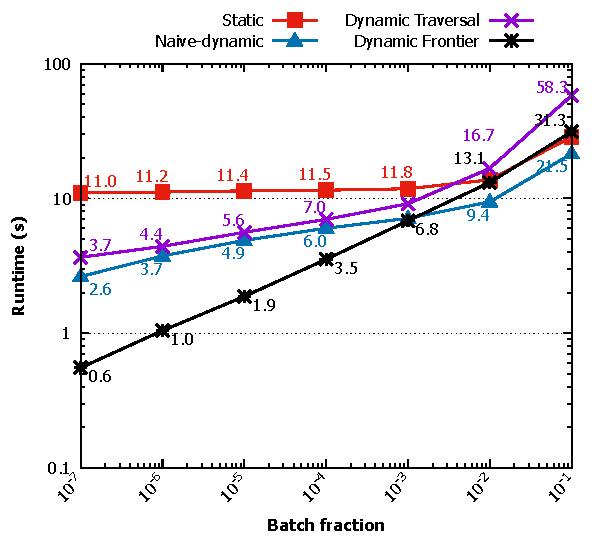
\includegraphics[width=0.38\linewidth]{out/insertions-runtime-mean.pdf}
  }
  \subfigure[Results on each graph]{
    \label{fig:insertions-runtime--all}
    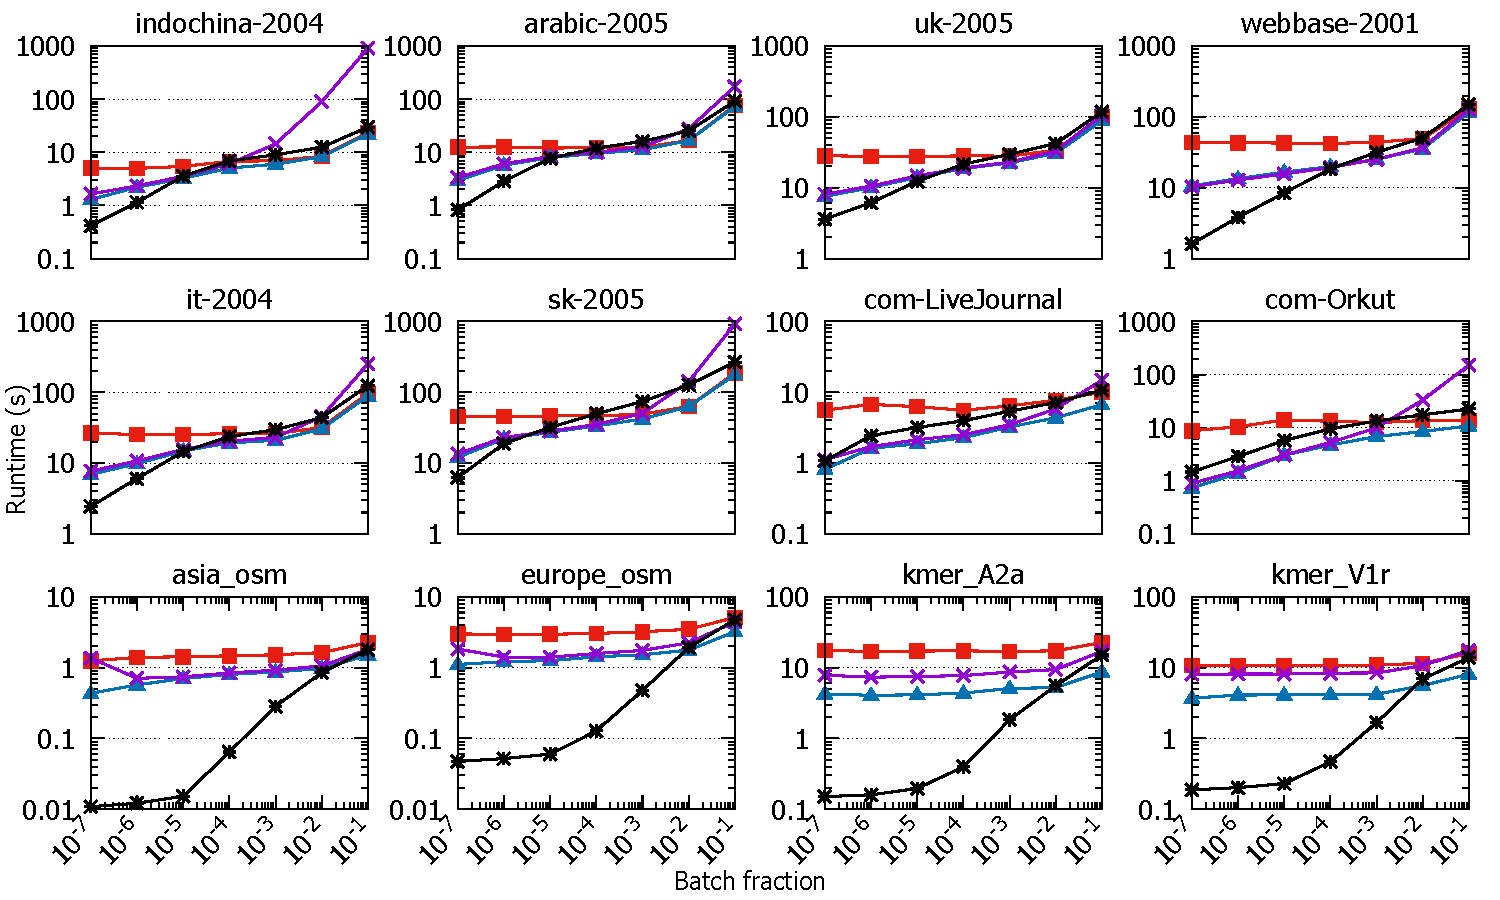
\includegraphics[width=0.58\linewidth]{out/insertions-runtime-all.pdf}
  } \\[-1ex]
  \caption{Runtime (logarithmic scale) for \textit{Static}, \textit{Naive-dynamic}, \textit{Dynamic Traversal}, and \textit{Dynamic Frontier} PageRank with batch updates exclusively comprising edge insertions, ranging from $10^{-7} |E|$ to $0.1 |E|$ in multiples of $10$ (logarithmic scale). The right figure details the runtime of each approach for individual graphs in the dataset, while the left figure displays overall runtimes --- using geometric mean for consistent scaling across graphs.}
  \label{fig:insertions-runtime}
\end{figure*}

\begin{figure*}[hbtp]
  \centering
  % \includegraphics[width=0.44\linewidth]{out/insertions-speedup-key.pdf}
  \subfigure[Overall result]{
    \label{fig:insertions-speedup--mean}
    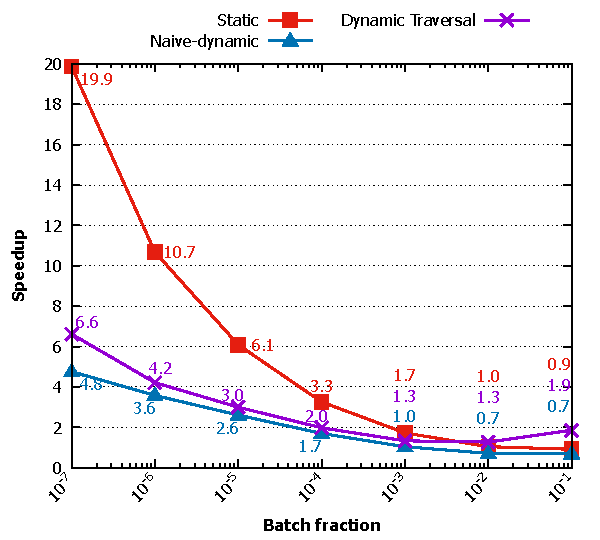
\includegraphics[width=0.38\linewidth]{out/insertions-speedup-mean.pdf}
  }
  \subfigure[Results on each graph]{
    \label{fig:insertions-speedup--all}
    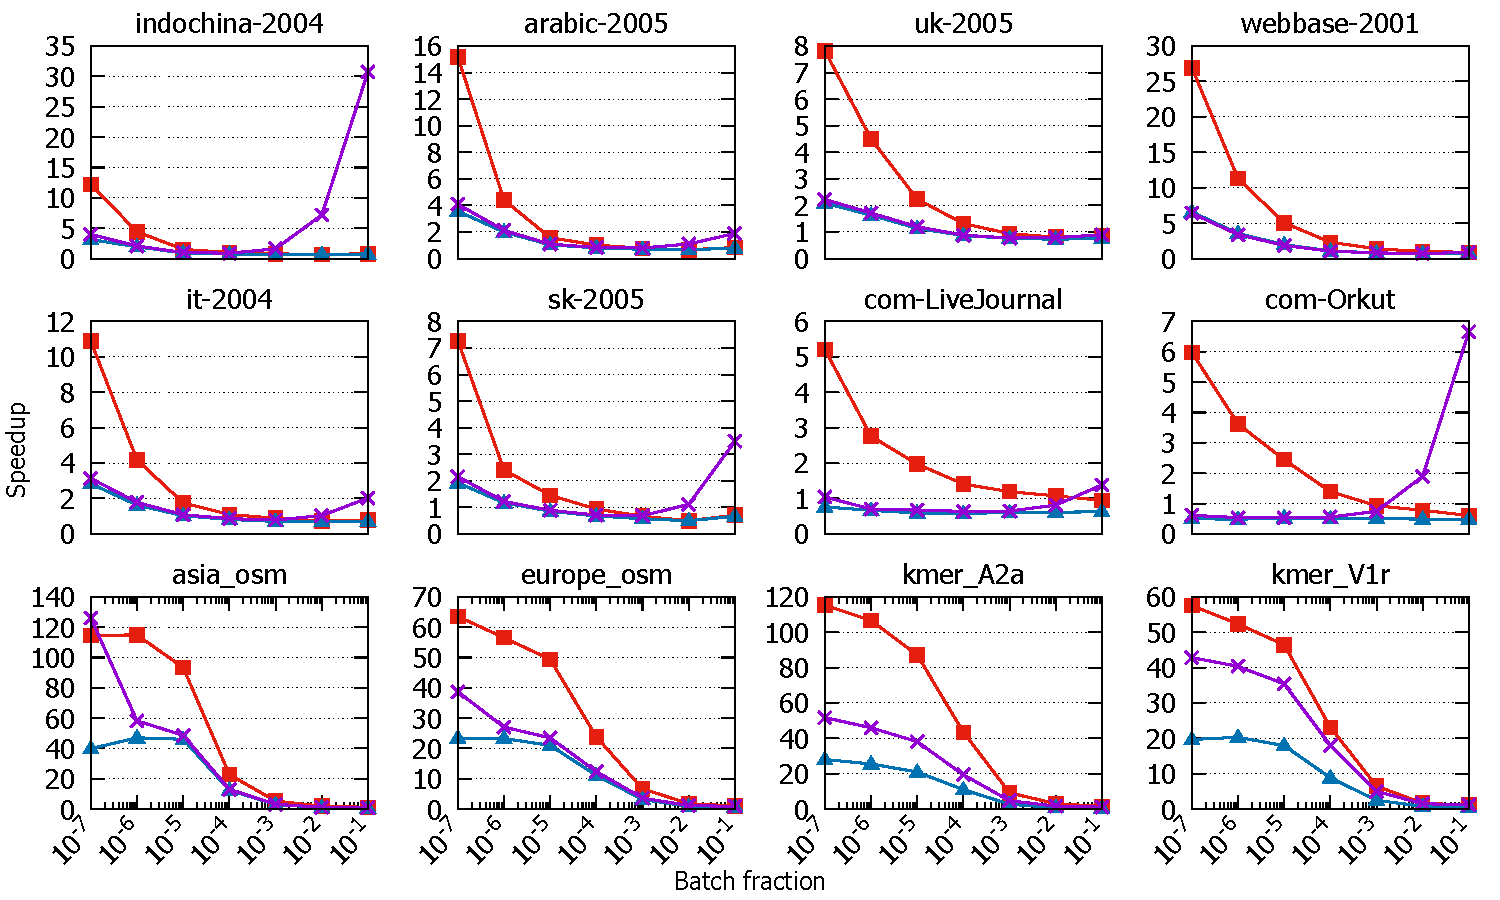
\includegraphics[width=0.58\linewidth]{out/insertions-speedup-all.pdf}
  } \\[-1ex]
  \caption{Speedup of \textit{Dynamic Frontier} PageRank with respect to \textit{Static}, \textit{Naive-dynamic}, and \textit{Dynamic Traversal} PageRank, on batch updates consisting solely of edge insertions ranging from $10^{-7} |E|$ to $0.1 |E|$ (logarithmic scale). The right figure depicts the speedup of \textit{Dynamic Frontier} PageRank in relation to each approach for individual graphs in the dataset, while the left figure highlights the overall speedup.}
  \label{fig:insertions-speedup}
\end{figure*}

\begin{figure*}[hbtp]
  \centering
  % \includegraphics[width=0.44\linewidth]{out/insertions-error-key.pdf}
  \subfigure[Overall result]{
    \label{fig:insertions-error--mean}
    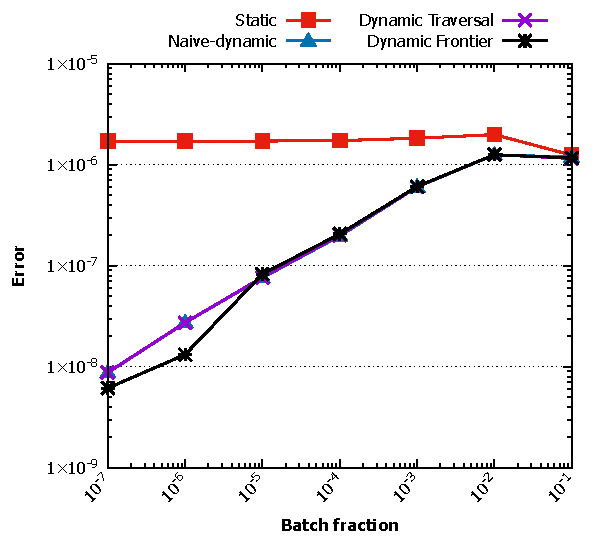
\includegraphics[width=0.38\linewidth]{out/insertions-error-mean.pdf}
  }
  \subfigure[Results on each graph]{
    \label{fig:insertions-error--all}
    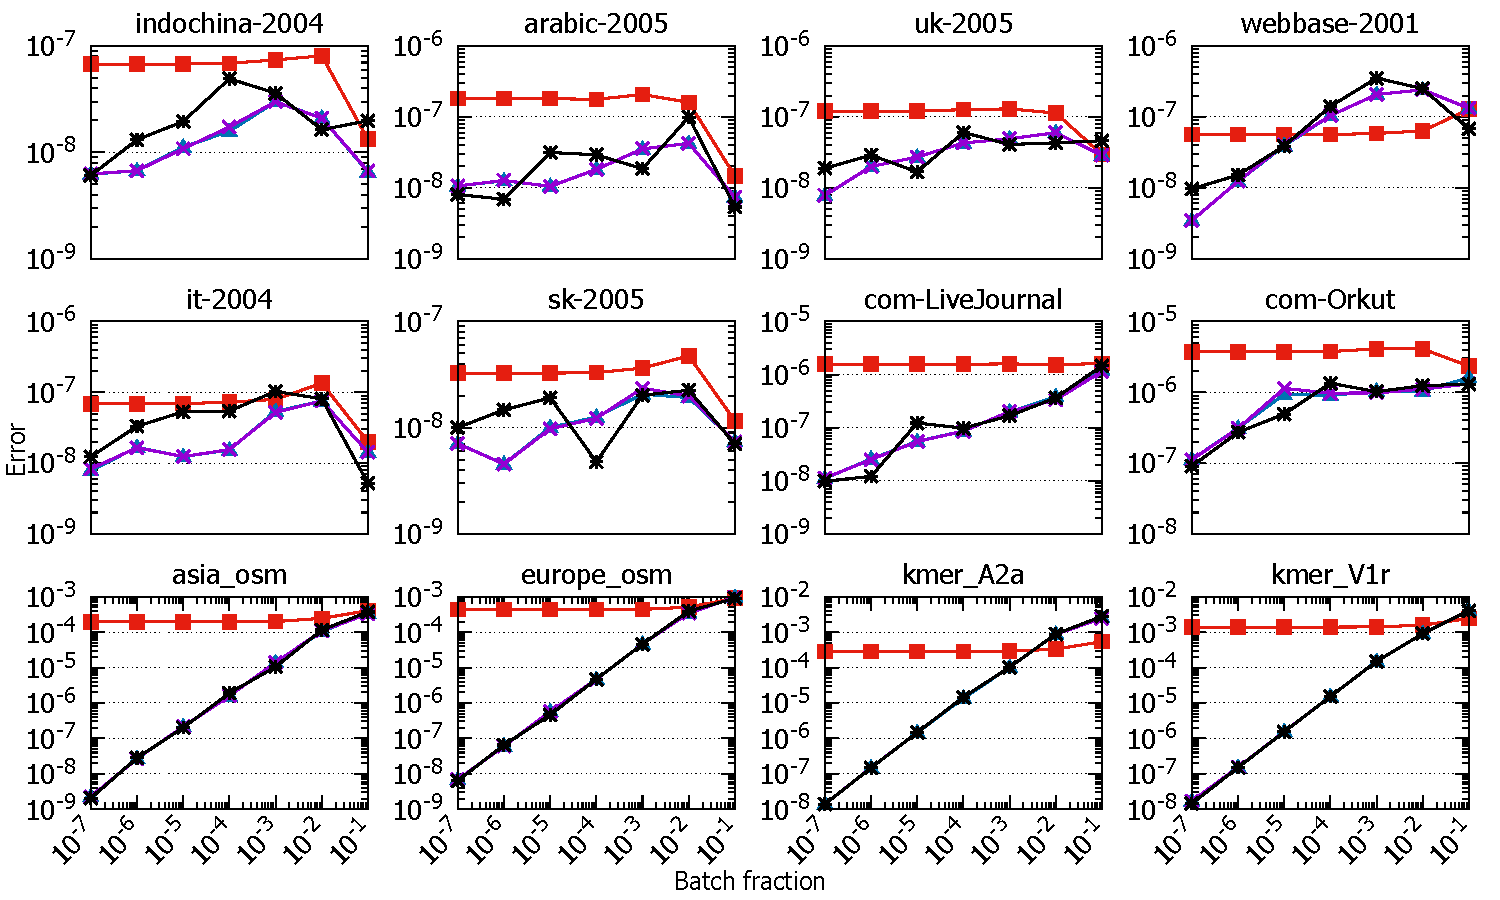
\includegraphics[width=0.58\linewidth]{out/insertions-error-all.pdf}
  } \\[-1ex]
  \caption{Error analysis comparing \textit{Static}, \textit{Naive-dynamic}, \textit{Dynamic Traversal}, and \textit{Dynamic Frontier} PageRank with a Reference Static PageRank (with a tolerance $\tau$ of $10^{-100}$ and limited to $500$ iterations) using $L1$-norm. Batch updates involve edge insertions ranging from $10^{-7} |E|$ to $0.1 |E|$ (logarithmic scale). The right figure illustrates the error specific to each approach for individual graphs in the dataset, while the left figure presents overall errors using the geometric mean for consistent scaling across graphs.}
  \label{fig:insertions-error}
\end{figure*}

\begin{figure*}[hbtp]
  \centering
  % \includegraphics[width=0.44\linewidth]{out/deletions-runtime-key.pdf}
  \subfigure[Overall result]{
    \label{fig:deletions-runtime--mean}
    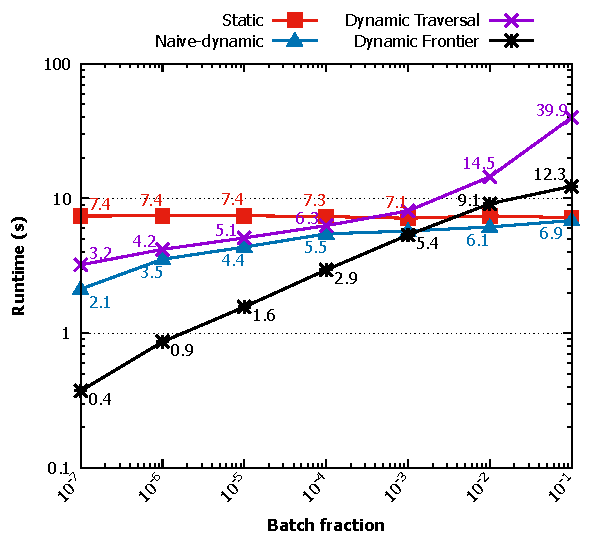
\includegraphics[width=0.38\linewidth]{out/deletions-runtime-mean.pdf}
  }
  \subfigure[Results on each graph]{
    \label{fig:deletions-runtime--all}
    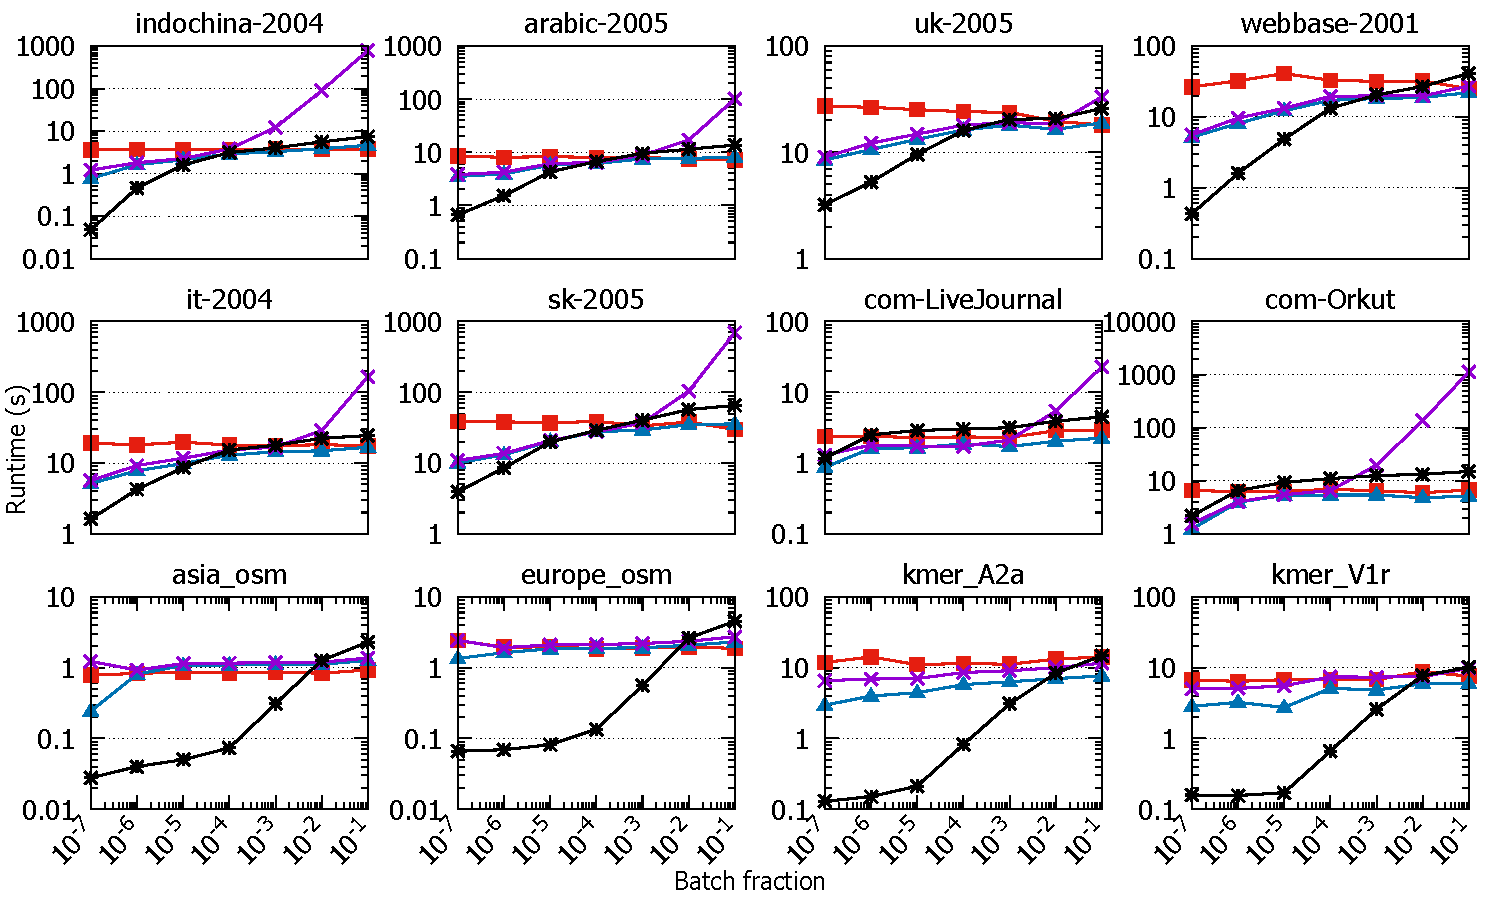
\includegraphics[width=0.58\linewidth]{out/deletions-runtime-all.pdf}
  } \\[-1ex]
  \caption{Deletions Time taken (solid lines), and modularity of communities obtained (dashed lines) along the Y2 axis, with X, X, and X (Algorithm X) on batch updates of increasing size from $10^{-7} |E|$ to $0.1 |E|$. Note that both axes are logarithmic. The numbers on the lines corresponding to X and X indicate the speedup of X over  the two algorithms, respectively.}
  \label{fig:deletions-runtime}
\end{figure*}

\begin{figure*}[hbtp]
  \centering
  % \includegraphics[width=0.44\linewidth]{out/deletions-speedup-key.pdf}
  \subfigure[Overall result]{
    \label{fig:deletions-speedup--mean}
    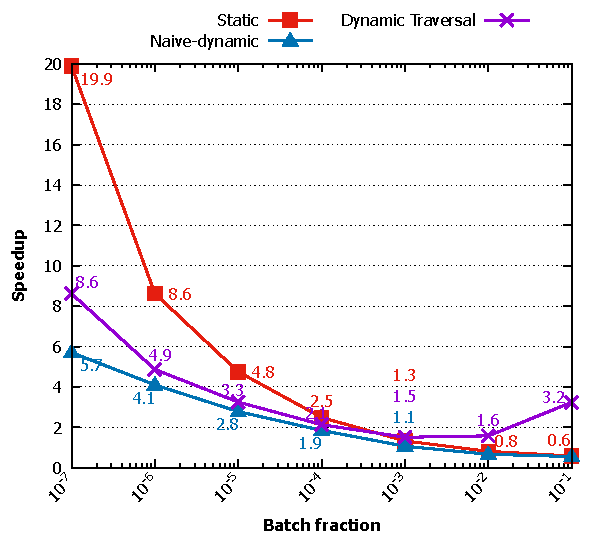
\includegraphics[width=0.38\linewidth]{out/deletions-speedup-mean.pdf}
  }
  \subfigure[Results on each graph]{
    \label{fig:deletions-speedup--all}
    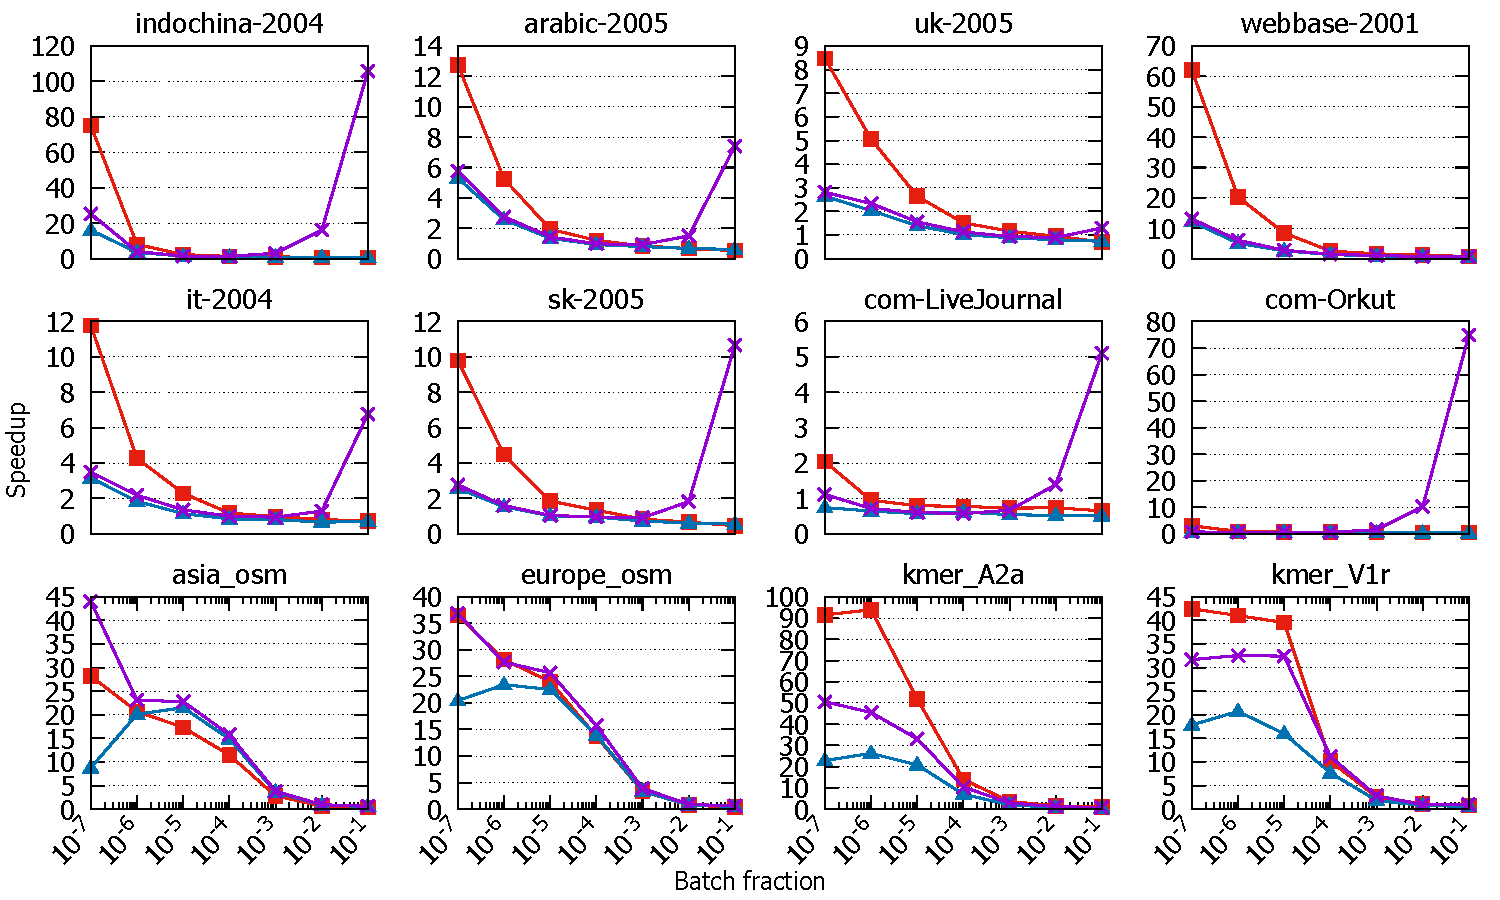
\includegraphics[width=0.58\linewidth]{out/deletions-speedup-all.pdf}
  } \\[-1ex]
  \caption{Speedup of \textit{Dynamic Frontier} PageRank in relation to \textit{Static}, \textit{Naive-dynamic}, and \textit{Dynamic Traversal} PageRank, on batch updates comprised solely of edge deletions ranging from $10^{-7} |E|$ to $0.1 |E|$ (logarithmic scale). The right figure illustrates the speedup of \textit{Dynamic Frontier} PageRank concerning each approach for individual graphs in the dataset, while the left figure emphasizes the overall speedup.}
  \label{fig:deletions-speedup}
\end{figure*}

\begin{figure*}[hbtp]
  \centering
  % \includegraphics[width=0.44\linewidth]{out/deletions-error-key.pdf}
  \subfigure[Overall result]{
    \label{fig:deletions-error--mean}
    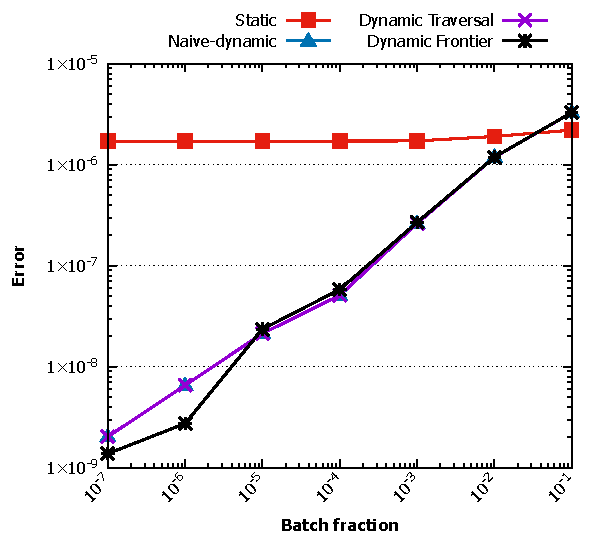
\includegraphics[width=0.38\linewidth]{out/deletions-error-mean.pdf}
  }
  \subfigure[Results on each graph]{
    \label{fig:deletions-error--all}
    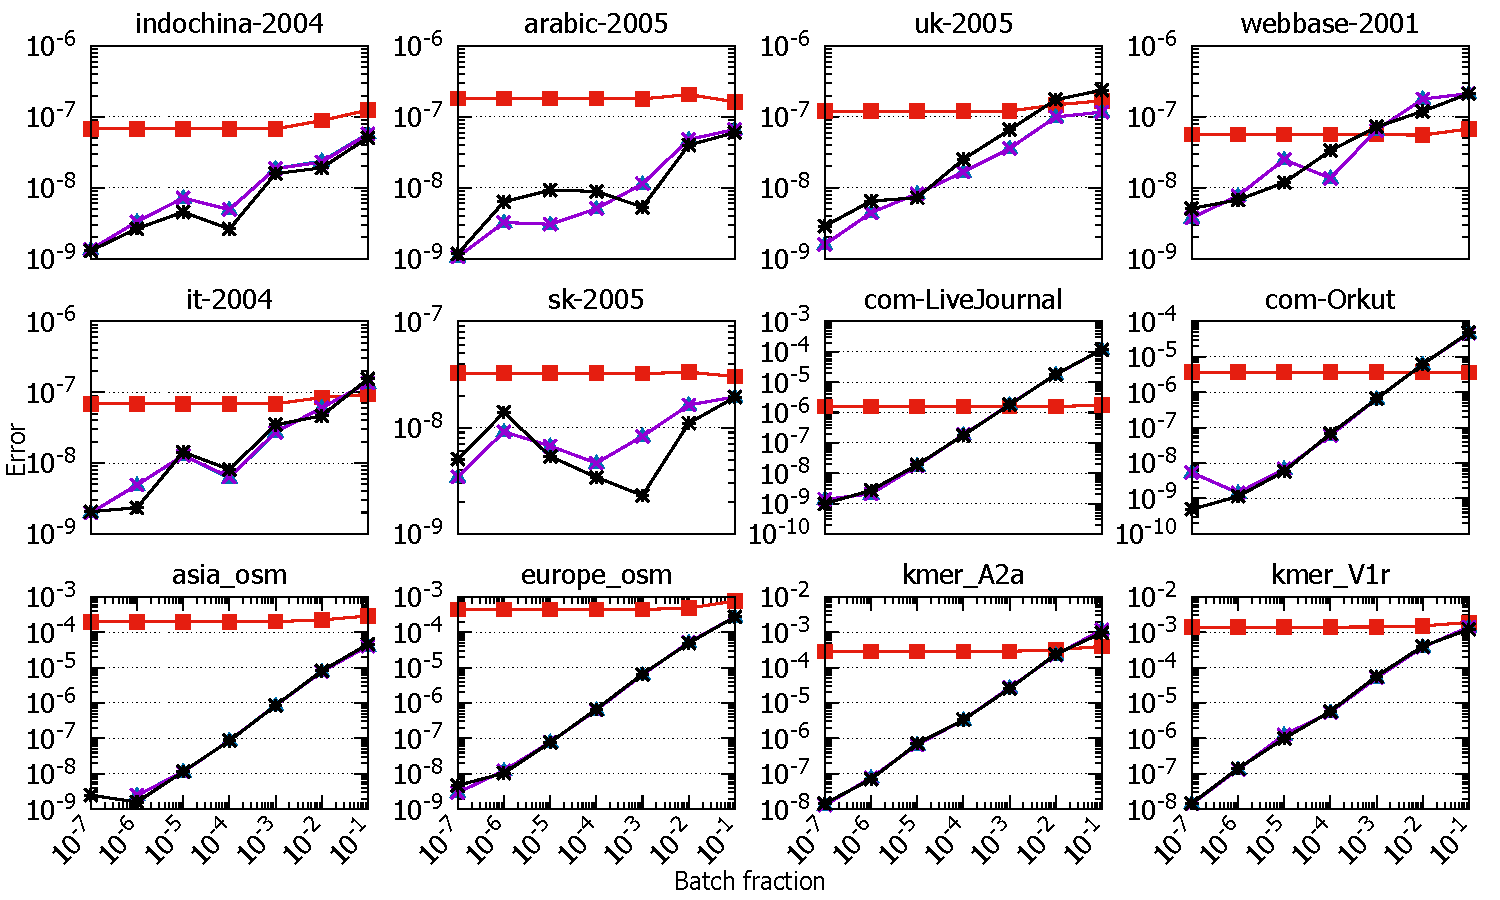
\includegraphics[width=0.58\linewidth]{out/deletions-error-all.pdf}
  } \\[-1ex]
  \caption{Deletions Time taken (solid lines), and modularity of communities obtained (dashed lines) along the Y2 axis, with X, X, and X (Algorithm X) on batch updates of increasing size from $10^{-7} |E|$ to $0.1 |E|$. Note that both axes are logarithmic. The numbers on the lines corresponding to X and X indicate the error of X over  the two algorithms, respectively.}
  \label{fig:deletions-error}
\end{figure*}

\begin{figure*}[hbtp]
  \centering
  % \includegraphics[width=0.44\linewidth]{out/8020-runtime-key.pdf}
  \subfigure[Overall result]{
    \label{fig:8020-runtime--mean}
    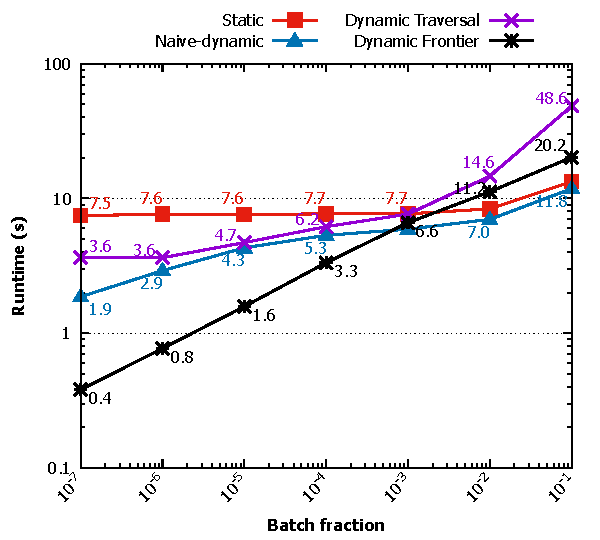
\includegraphics[width=0.38\linewidth]{out/8020-runtime-mean.pdf}
  }
  \subfigure[Results on each graph]{
    \label{fig:8020-runtime--all}
    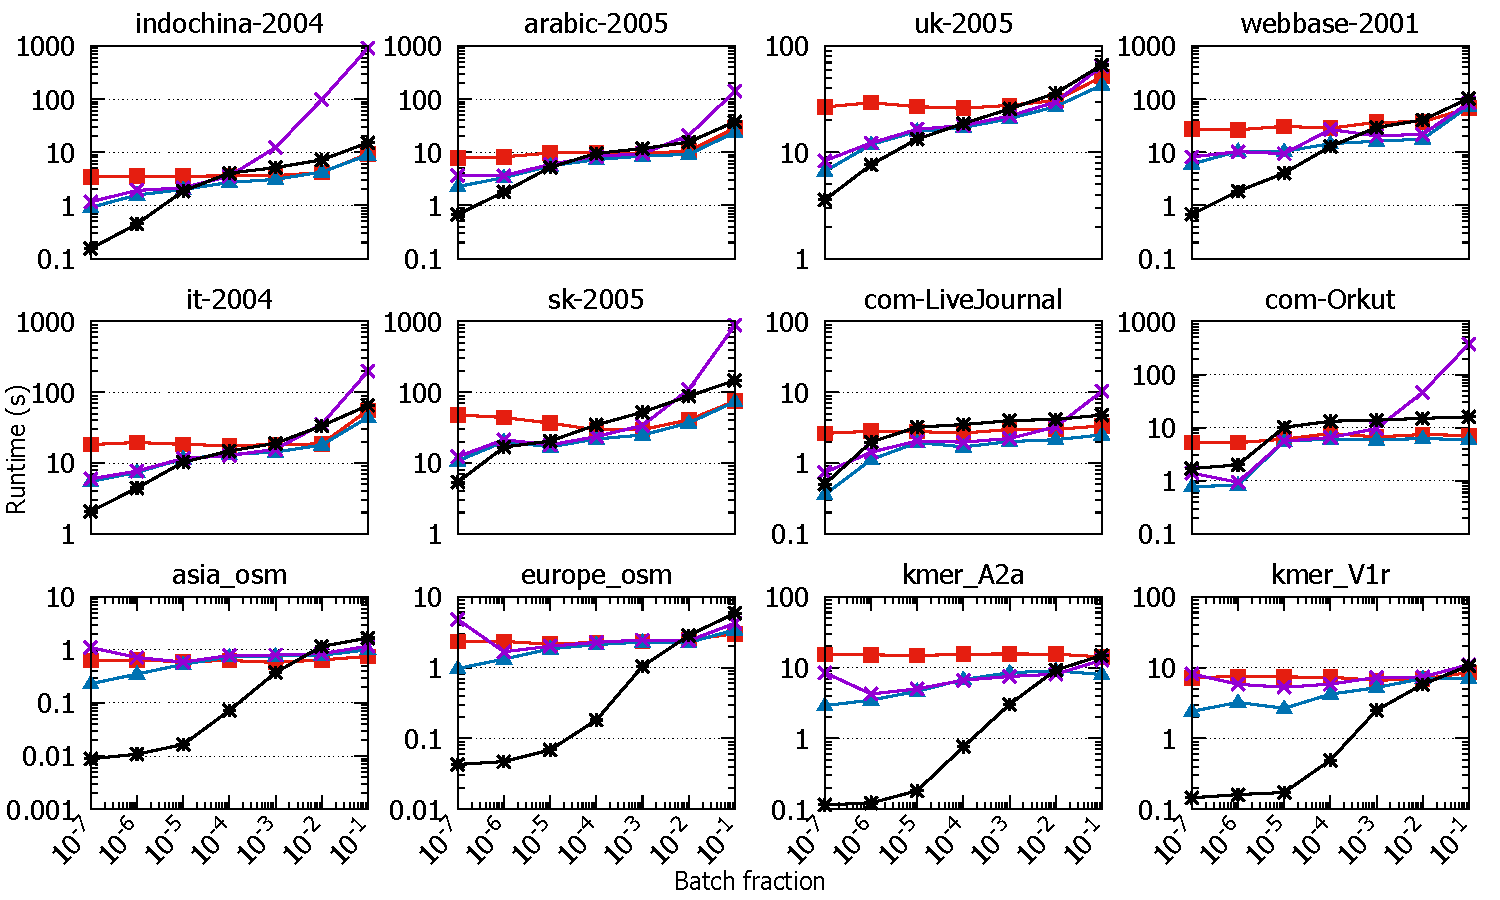
\includegraphics[width=0.58\linewidth]{out/8020-runtime-all.pdf}
  } \\[-1ex]
  \caption{8020 Time taken (solid lines), and modularity of communities obtained (dashed lines) along the Y2 axis, with X, X, and X (Algorithm X) on batch updates of increasing size from $10^{-7} |E|$ to $0.1 |E|$. Note that both axes are logarithmic. The numbers on the lines corresponding to X and X indicate the speedup of X over  the two algorithms, respectively.}
  \label{fig:8020-runtime}
\end{figure*}

\begin{figure*}[hbtp]
  \centering
  % \includegraphics[width=0.44\linewidth]{out/8020-speedup-key.pdf}
  \subfigure[Overall result]{
    \label{fig:8020-speedup--mean}
    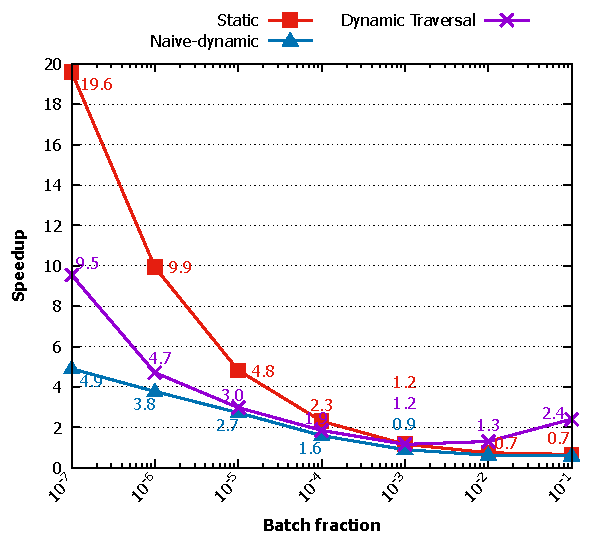
\includegraphics[width=0.38\linewidth]{out/8020-speedup-mean.pdf}
  }
  \subfigure[Results on each graph]{
    \label{fig:8020-speedup--all}
    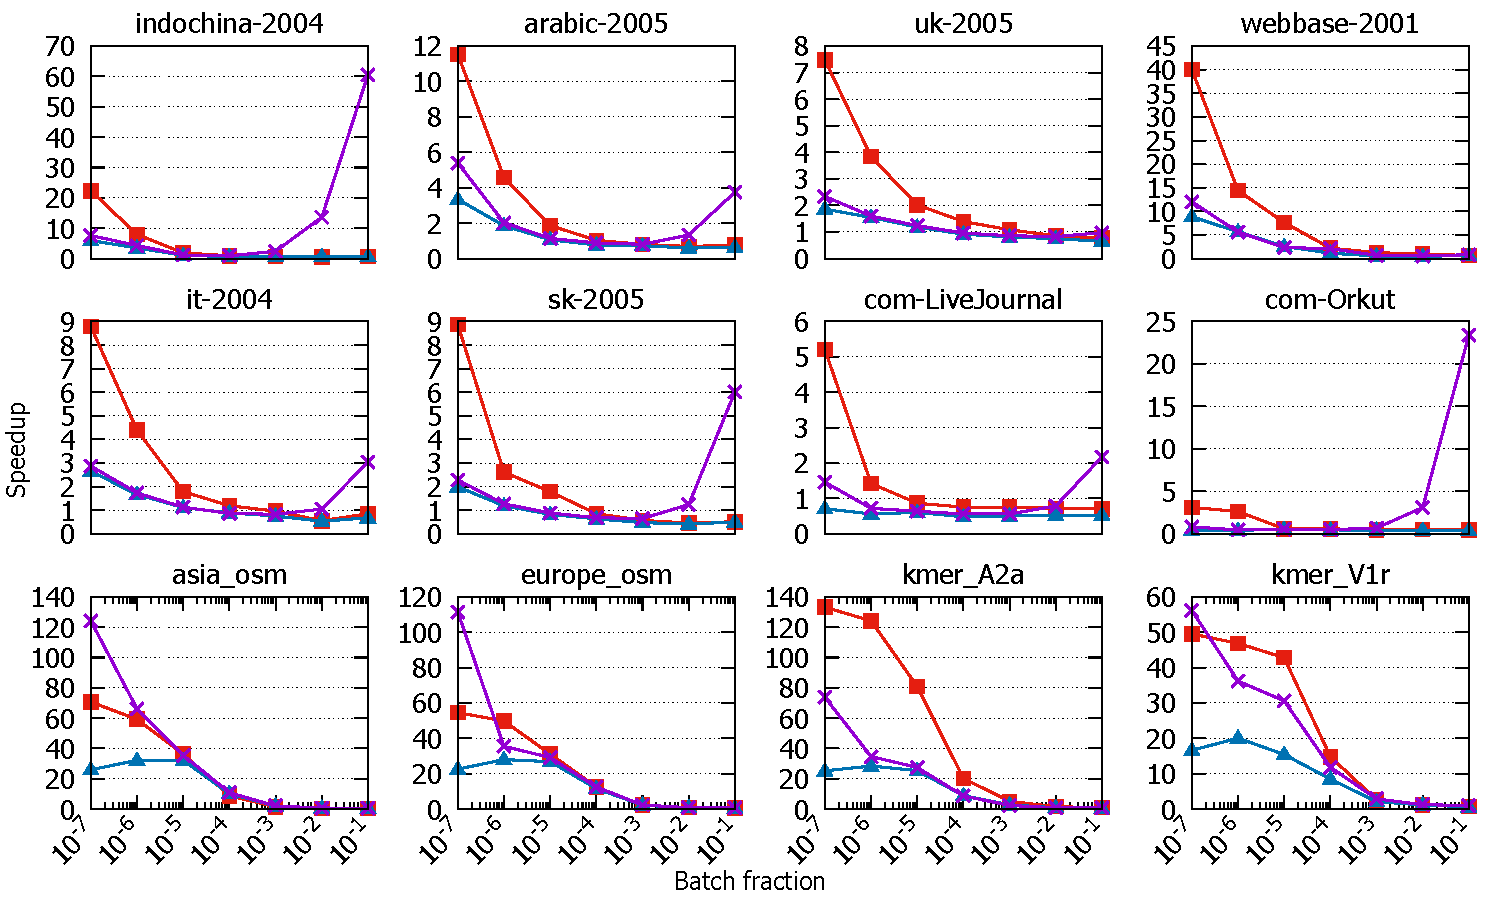
\includegraphics[width=0.58\linewidth]{out/8020-speedup-all.pdf}
  } \\[-1ex]
  \caption{8020 Time taken (solid lines), and modularity of communities obtained (dashed lines) along the Y2 axis, with X, X, and X (Algorithm X) on batch updates of increasing size from $10^{-7} |E|$ to $0.1 |E|$. Note that both axes are logarithmic. The numbers on the lines corresponding to X and X indicate the speedup of X over  the two algorithms, respectively.}
  \label{fig:8020-speedup}
\end{figure*}

\begin{figure*}[hbtp]
  \centering
  % \includegraphics[width=0.44\linewidth]{out/8020-error-key.pdf}
  \subfigure[Overall result]{
    \label{fig:8020-error--mean}
    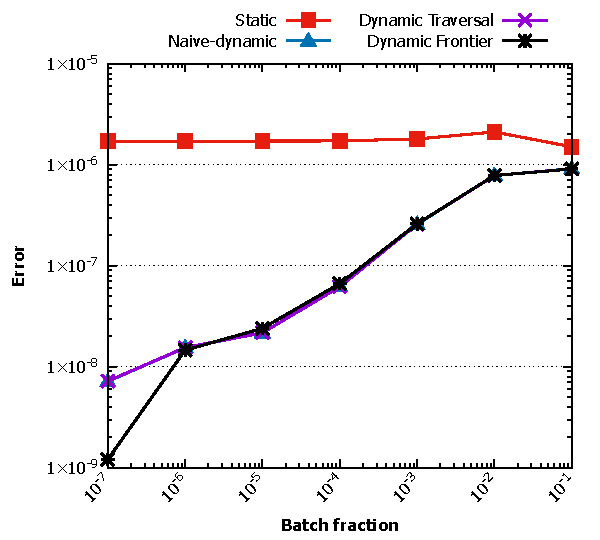
\includegraphics[width=0.38\linewidth]{out/8020-error-mean.pdf}
  }
  \subfigure[Results on each graph]{
    \label{fig:8020-error--all}
    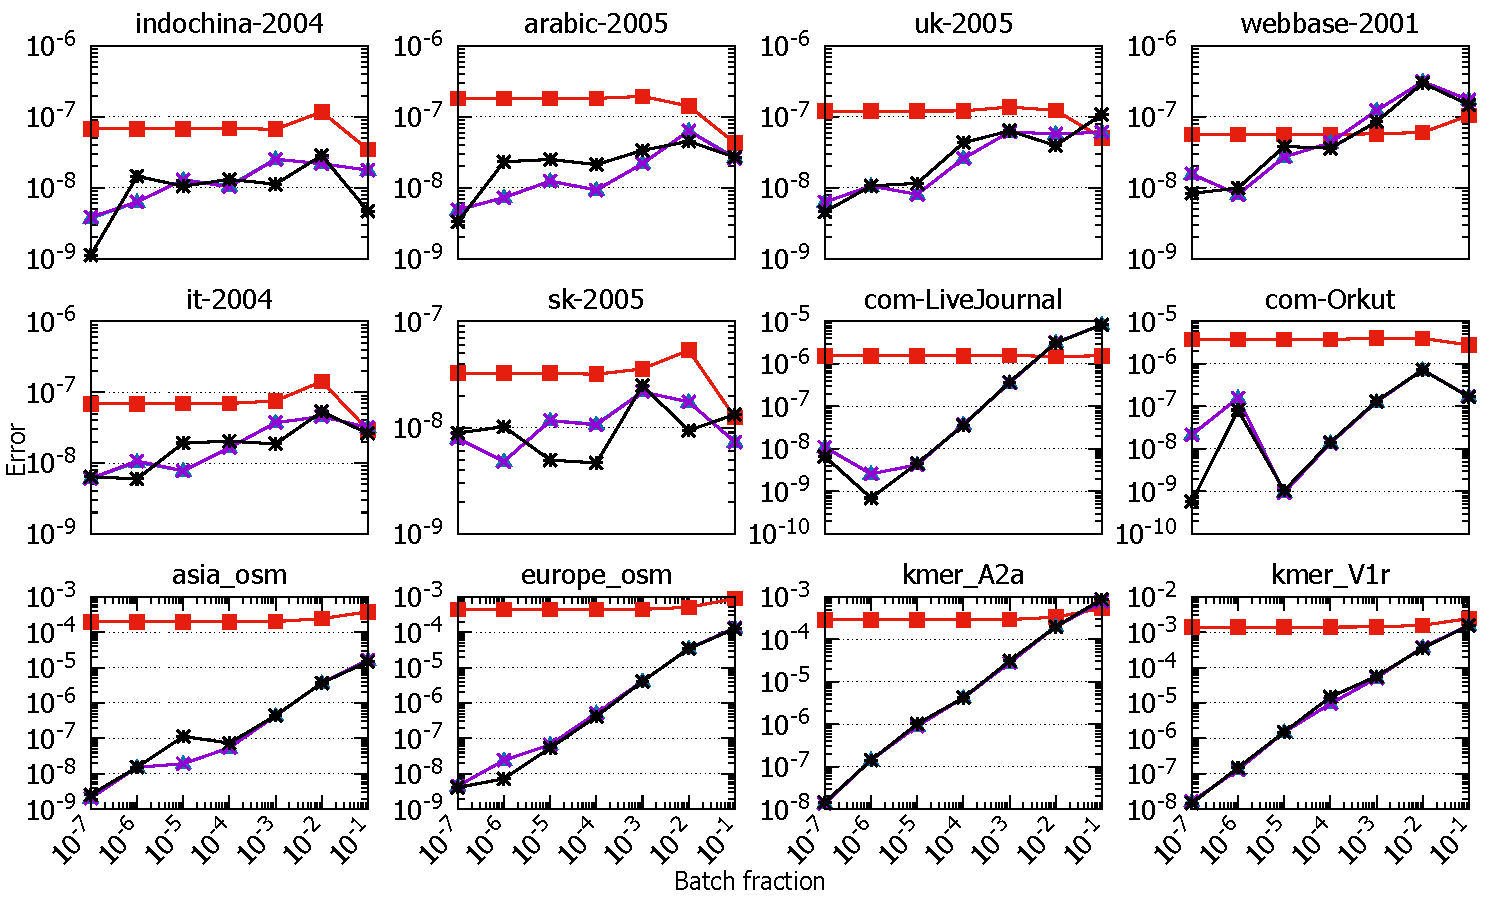
\includegraphics[width=0.58\linewidth]{out/8020-error-all.pdf}
  } \\[-1ex]
  \caption{Error comparison of \textit{Static}, \textit{Naive-dynamic}, \textit{Dynamic Traversal}, and \textit{Dynamic Frontier} PageRank with respect to a Reference Static PageRank (with a tolerance $\tau$ of $10^{-100}$ and limited to $500$ iterations), using $L1$-norm. Batch updates range from $10^{-7} |E|$ to $0.1 |E|$ (logarithmic scale), consisting of $80\%$ edge insertions and $20\%$ edge deletions to simulate realistic dynamic graph updates. The right figure depicts the error for each approach in relation to each graph, while the left figure showcases overall errors using geometric mean for consistent scaling across graphs.}
  \label{fig:8020-error}
\end{figure*}

\begin{figure}[!hbt]
  \centering
  \subfigure{
    \label{fig:measure-affected--batch}
    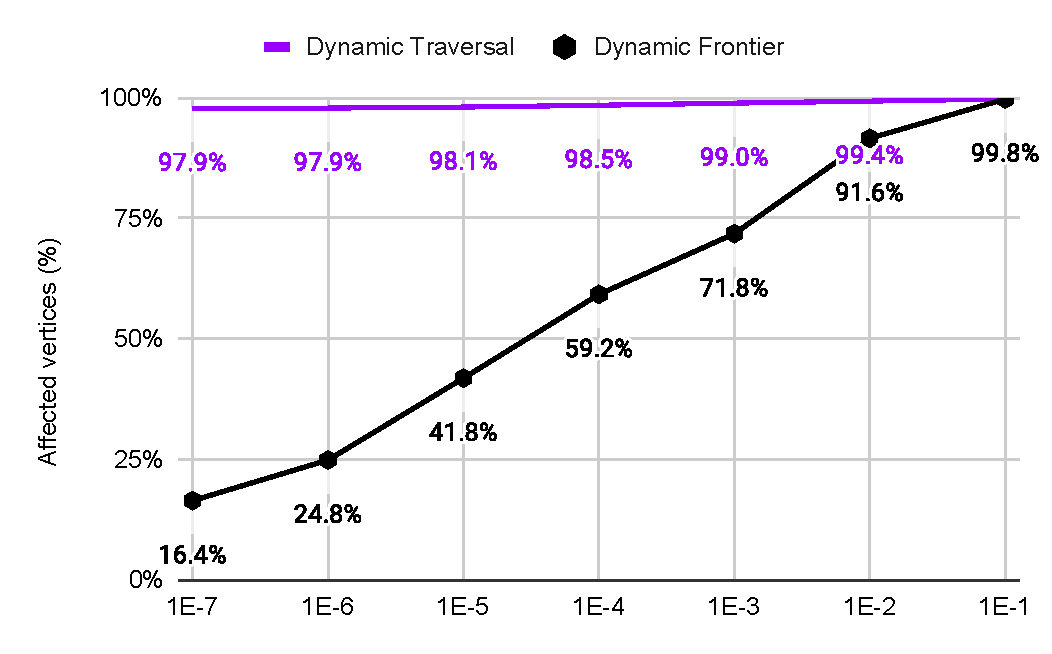
\includegraphics[width=0.98\linewidth]{out/measure-affected-batch.pdf}
  } \\[-2ex]
\caption{Average percentage of vertices marked as affected by \textit{Dynamic Traversal} and \textit{Dynamic Frontier} PageRank, with batch size increasing from $10^{-7} |E|$ to $0.1 |E|$ in multiples of $10$ (logarithmic scale), consisting purely of edge insertions. The \textit{Dynamic Frontier} approach marks affected vertices incrementally --- thus, the final percentage (at the end of all iterations) is depicted here.}
  \label{fig:measure-affected}
\end{figure}





\subsection{Strong Scaling of DF-PageRank}

Finally, we study the strong-scaling behavior of \textit{Dynamic Frontier} PageRank on batch updates of a fixed size of $10^{-4} |E|$, consisting purely of edge insertions. Here, we measure the speedup of \textit{Dynamic Frontier} PageRank with an increasing number of threads from $1$ to $64$ in multiples of $2$ with respect to a single-threaded execution of the algorithm. This is repeated to each graph in the dataset, and the results are averaged (using geometric mean).

The results are shown in Figure \ref{fig:strong-scaling}. With $16$ threads, \textit{Dynamic Frontier} PageRank achieves an average speedup of $10.3\times$, compared to a single-threaded execution, indicating a performance increase of $1.8\times$ for every doubling of threads. At $32$ and $64$ threads, \textit{Dynamic Frontier} PageRank is affected by NUMA effects (the $64$-core processor we use has $4$ NUMA domains), resulting in a speedup of only $14.3\times$ and $15.2\times$ respectively.

\begin{figure}[!hbt]
  \centering
  \subfigure{
    \label{fig:strong-scaling--speedup}
    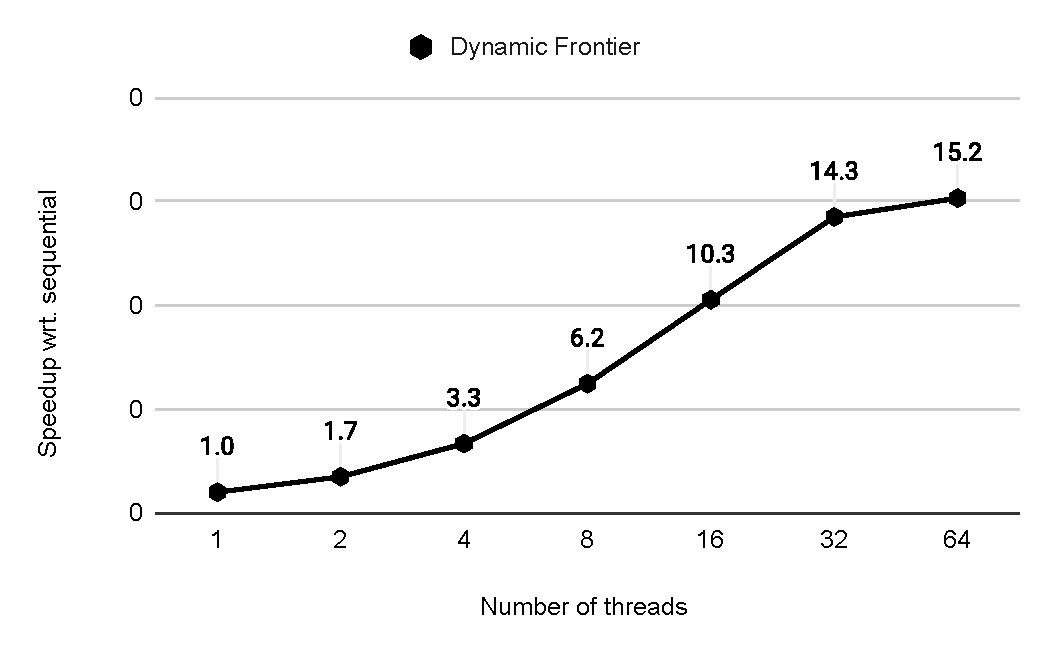
\includegraphics[width=0.98\linewidth]{out/strong-scaling-speedup.pdf}
  } \\[-2ex]
  \caption{Average speedup of \textit{Dynamic Frontier} PageRank with increasing number of threads (in multiples of $2$), on a batch size of $10^{-4}|E|$ (consisting purely of edge insertions).}
  \label{fig:strong-scaling}
\end{figure}

\ignore{\begin{figure}[!hbt]
  \centering
  \subfigure{
    \label{fig:weak-scaling--speedup}
    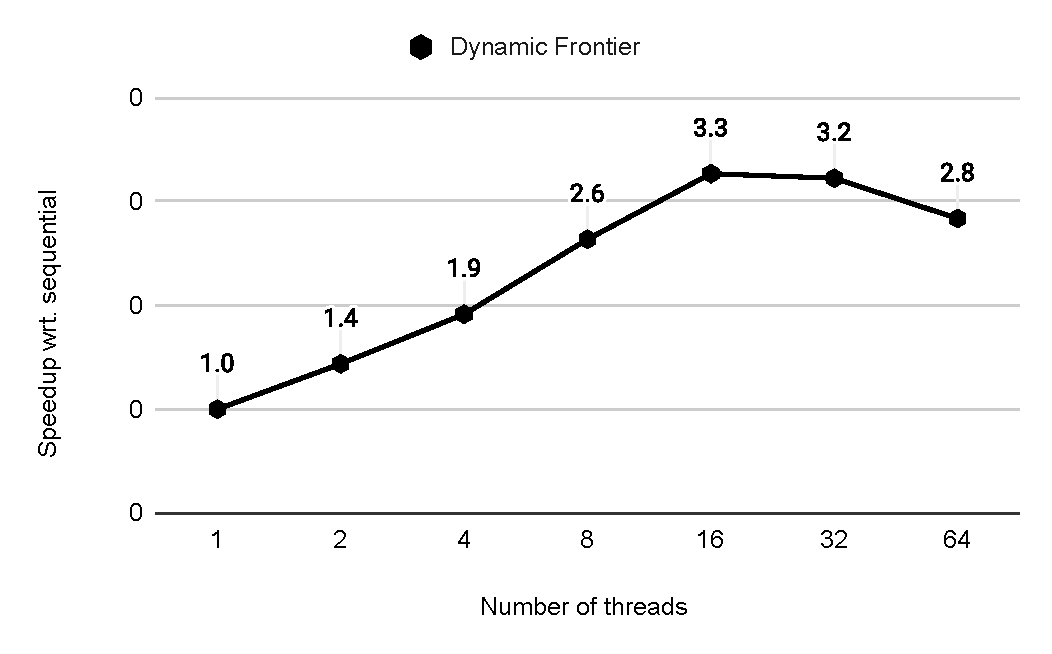
\includegraphics[width=0.98\linewidth]{out/weak-scaling-speedup.pdf}
  } \\[-2ex]
  \caption{Average speedup of \textit{Dynamic Frontier} PageRank with increasing number of threads (in multiples of $2$), on a batch sizes of $10^{-4}|E|$ to $6.4\times10^{-3}|E|$ (consisting purely of edge insertions), increasing in multiples of $2$ in tandem with the increase in the number of threads.}
  \label{fig:weak-scaling}
\end{figure}
}
